\section{Single Qubit Readout on QICK System}
{{\footnotesize
\begin{description}[labelwidth=5em, labelsep=1em, leftmargin=*, align=left, itemsep=0.3em, parsep=0em]
  \item[date:] 2025-01-24
  \item[version:] TODO
  \item[last\_updated:] 2025-02
  \item[expired:] unknown
  \item[valid:] yes
  \item[valid\_date:] TODO
  \item[url:] \href{https://github.com/fastmachinelearning/ml-quantum-readout}{https://github.com/fastmachinelearning/ml-quantum-readout}
  \item[doi:] TODO
  \item[domain:] Quantum Computing
  \item[focus:] Real-time single-qubit state classification using FPGA firmware
  \item[keywords:]
    - qubit readout
    - hls4ml
    - FPGA
    - QICK
  \item[summary:] Implements real-time ML models for single-qubit readout on the Quantum Instrumentation Control Kit (QICK), using hls4ml to deploy quantized neural networks on RFSoC FPGAs. Offers high-fidelity, low-latency quantum state discrimination. :contentReference[oaicite:0]\{index=0\}

  \item[licensing:] TODO
  \item[task\_types:]
    - Classification
  \item[ai\_capability\_measured:]
    - Single-shot fidelity
    - inference latency
  \item[metrics:]
    - Accuracy
    - Latency
  \item[models:]
    - hls4ml quantized NN
  \item[ml\_motif:]
    - Real-time
  \item[type:] Benchmark
  \item[ml\_task:]
    - Supervised Learning
  \item[solutions:] TODO
  \item[notes:] Achieves \textasciitilde{}96\% fidelity with \textasciitilde{}32 ns latency and low FPGA resource utilization. :contentReference[oaicite:1]\{index=1\}

  \item[contact.name:] Javier Campos, Giuseppe Di Guglielmo
  \item[contact.email:] unknown
  \item[datasets.links.name:] Zenodo: ml-quantum-readout dataset
  \item[datasets.links.url:] \href{zenodo.org/records/14427490}{zenodo.org/records/14427490}
  \item[results.links.name:] ChatGPT LLM
  \item[fair.reproducible:] Yes
  \item[fair.benchmark\_ready:] Yes
  \item[ratings.software.rating:] 0
  \item[ratings.software.reason:] Not analyzed.

  \item[ratings.specification.rating:] 8.0
  \item[ratings.specification.reason:] Task clearly framed around detecting hybrid species via images, but exact labeling methods and hybrid definitions may need elaboration.

  \item[ratings.dataset.rating:] 8.0
  \item[ratings.dataset.reason:] Dataset hosted on Codabench; appears structured but details on image sourcing and labeling pipeline are limited.

  \item[ratings.metrics.rating:] 9.0
  \item[ratings.metrics.reason:] Classification accuracy and F1 are standard and appropriate.

  \item[ratings.reference\_solution.rating:] 1.0
  \item[ratings.reference\_solution.reason:] No starter model or baseline code linked

  \item[ratings.documentation.rating:] 7.5
  \item[ratings.documentation.reason:] Codabench task page describes dataset and evaluation method but lacks full API/docs.

  \item[id:] single\_qubit\_readout\_on\_qick\_system
  \item[Citations:] \cite{diguglielmo2025endtoendworkflowmachinelearningbased}
  \item[Ratings:]
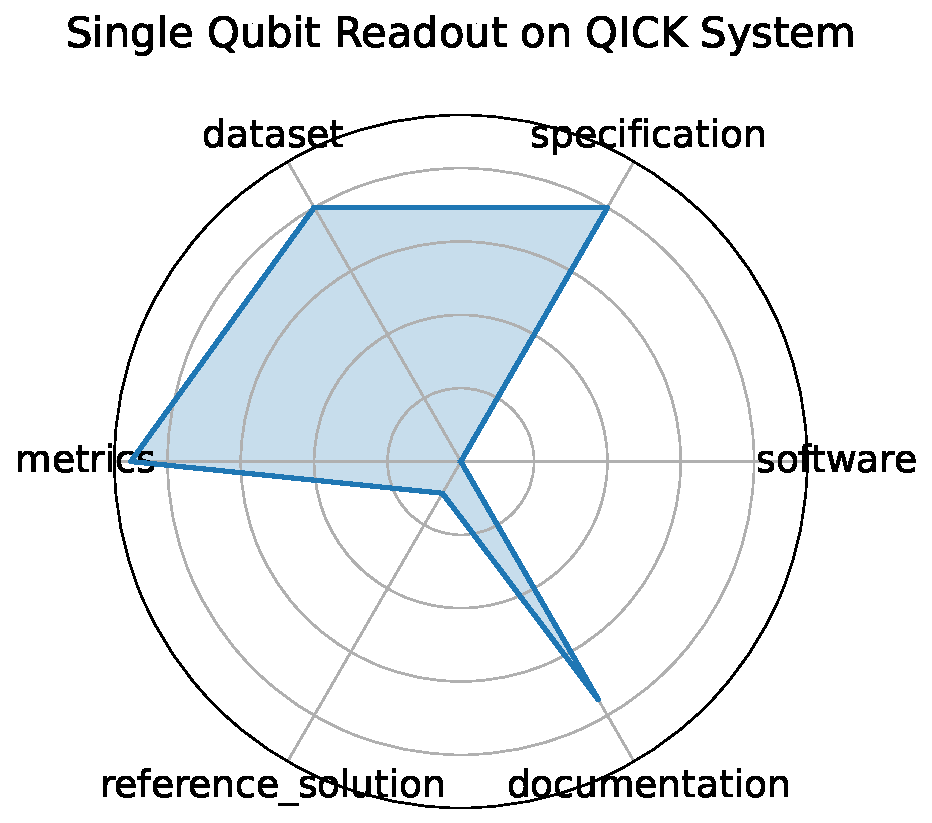
\includegraphics[width=0.2\textwidth]{single_qubit_readout_on_qick_system_radar.pdf}
\end{description}
}}
\clearpage